\documentclass[doctor]{snuece-bs}

\usepackage{biblatex}
\usepackage{comment}
\usepackage{algorithm}
\usepackage{algpseudocode}


\newcommand{\specialcell}[2][c]{%
  \begin{tabular}[#1]{@{}c@{}}#2\end{tabular}}

\addbibresource{10-bibliography.tex}

\title[korean]{AmslerTouch: 노인황반변성 증상의 정량적 자가진단을 지원하는 암슬러 그리드 애플리케이션 설계}
\title[english]{AmslerTouch: Self-testing Amsler Grid Application for Supporting a Quantitative Report of Age-related Macular Degeneration Symptoms}


\author[korean]{신 동 훈}
\author[english]{DONGHOON SHIN}
\author[nospace]{신동훈}


\advisor{서 종 모}

\submissiondeadline{2021년 6월}
\examinationdate{2021년 8월}

\gradyear[english]{AUGUST 2022}
\gradyear[korean]{2022년 8월}


\begin{document}
\renewcommand{\baselinestretch}{1.5}

\selectfont

\begin{abstract}
	\par
	Age-related macular degeneration (AMD) is a progressive chronic disease that is led by damage in the macula. Due to its irreversible characteristics and disastrous effects on the patients, a precise diagnosis of the symptoms is extremely important. Yet, paper-based Amsler Grid, the most prevalent testing method, is highly limited in that it requires the indirect report of patients and quantitative reporting is difficult. To address this, I propose AmslerTouch, a touch-based Amsler-testing web app that supports patients to self-report AMD symptoms. Based on the heuristic evaluation for identifying limitations and gaining insights, I also discuss possible enhancements of my proposed system.
	\vfill
	\begin{minipage}[t][20mm][b]{\textwidth}
		{\bfseries Keywords}: Age-related Macular Degeneration, Amsler Grid, Healthcare\\
		{\bfseries Student number}: 2016-16578\\
	\end{minipage}
	
\end{abstract}

\changepage{5mm}{}{}{}{}{}{}{}{-5mm}

\makelists

\chapter{INTRODUCTION}

Age-related macular degeneration (AMD) is a progressive chronic disease that is led by the damage in the macula~\cite{lim2012age}. According to Jeon et al., AMD is a highly prevalent disease in the society, where 6.62\% of South Korean population are suffering from the symptoms of AMD~\cite{park2014age}. It is widely known that the symptom often accompanies a disastrous symptoms, such as blurred vision or vision loss~\cite{lim2012age}. In addition to its detrimental effects on the vision itself, older adults with AMD are also prone to be affected psychologically, such as being depressed from the isolation from the society led by the symptom~\cite{rovner2007preventing}.

To date, however, little or no effective treatment for treating AMD exists~\cite{wong2011prevention}. Although some promising approaches such as stem cell implant have been proposed~\cite{carr2013development}, these methods are still yet to be widely applied. Thus, considering that it is almost impossible to revert once the degeneration is exacerbated, the most feasible and cost-effective management of AMD is to prevent further development of symptoms~\cite{al2017recent}, implying the necessity of the early detection and precise diagnosis of AMD.

As such, the importance of precise diagnosis has been highly emphasized so far. Yet, most of the diagnosis of AMD are limited in precisely reporting the region of issue. Specifically, patients and practitioners who conduct Amsler grid testing, the most prevalent AMD testing since 1940s, often suffer from the communicative issues, thus limiting the validity of the test~\cite{schuchard1993validity}. Heavily relying on the indirect, verbal report of patients, the regions of issue are often inexactly reported, making such symptoms difficult to be accurately managed.

In order to address such an issue, I propose a novel application of self-reporting symptoms of AMD with Amsler grid. Specifically, based on the literature review of AMD and the symptoms that are led by the disease, I developed AmslerTouch, a touch-based Amsler-testing web app that supports patients to self-report AMD symptoms. AmslerTouch supports users to precisely annotate regions of symptoms. As such, I aimed to faciliated decision making of practitioners with the quantitative report of AMD symptoms with a widely-available tablet device. Based on the reflection on AmslerTouch, I also discuss possible enhancements and future works.

\chapter{BODY}

\section{Method}
This study was built upon the previous works in the field of medicine and human-computer interaction (HCI) that dealt with diagnosing AMD symptoms with aids of computing systems. Based on the implications of these approaches and the understanding of frequent symptoms reported by ophthalmologists, I propose my touch-based interactive Amsler grid testing app.


\section{Literature Review}

\subsection{Diagnosis and Management of Symptoms with Aid of Computers}

With the advent and distribution of personal computing devices, previous studies have explored and proposed various computer-based techniques that supports diagnosis of various diseases and disorders. For example, Shin and his colleagues TalkingBoogie, a mobile app that supports ad hoc notes of communicative issues that children with non-verbal developmental disabilities show~\cite{shin2020talkingboogie}. Salai and Baillie developed a mobile application for recording overactive bladder symptoms~\cite{salai2019wee}.

\subsection{Age-related Macular Degeneration (AMD)}

\subsubsection{Distortion}

\begin{figure}[h!]
    \centering
    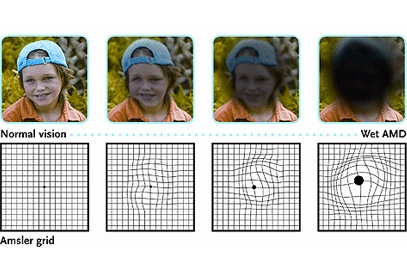
\includegraphics[width=0.6\linewidth]{figure/symptoms.jpg}
    \caption{Distortion}
    \label{fig:my_label}
\end{figure}

\subsection{Computer-based AMD Diagnosis}

Previous studies in the field of Human-computer interaction, bioengineering, and health informatics have explored several techniques that support medical practitioners and patients to diagnose symptoms of AMD in computers. Noting that paper-based AMD testing had been shown unsuccessful in terms of precise diagnosis~\cite{fine1986earliest, roy1985vision}, these studies emphasized the feasibility of computer-based approach for the precise and quantitative report of symptoms.

For example, Loewenstein et al. proposed MCPT, a system that supports patients to draw their region of symptoms on the computer~\cite{loewenstein2003replacing}. With basic input sources such as ordinary mouse and keyboard, these researchers sought to support a precise computer-based diagnosis. Mohaghegh and his colleagues developed a wearable system for diagnosing AMD symptoms~\cite{mohaghegh2016wearable}. They developed NGRID, a diagnosis system with a head-mounted device to support more precise diagnosis of AMD. In addition to such approaches, recent advent of 3D technologies made it possible to diagnose with 3D screen and glasses~\cite{kim2020novel}.

\begin{table}[htbp]
	\begin{center}
		\begin{tabular}{|c|c|} \hline
			Name & Description\\ \hline
			\hline {\sc MCPT~\cite{loewenstein2003replacing}} & Drawing on the computer with ordinary mouse and keyboard\\
			\hline {\sc NGRID~\cite{mohaghegh2016wearable}} & Head-mounted Amsler-grid app\\
			\hline {\sc 3D Test~\cite{kim2020novel}} & Implemented with 3D screen and polarized glasses\\
			\hline
		\end{tabular}
		\caption{Examples of AMD Diagnosis apps}
		\label{tab1}
	\end{center}
\end{table}

As such, previous researchers were successful in exploring design spaces of novel diagnosis systems and proposing them. Yet, these approaches are limited in its efficiency and generalizability, since (i) they only made use of simple input devices that might not be sufficient in terms of accuracy or (ii) the techniques required costly devices that are not easily available. With recent distribution of touch-based tablets, I found that these devices might give people a great opportunity to precisely note regions of symptom without purchasing any costly device. Thus, in this study, I propose an AMD diagnosis app that lets users easily utilize within their hand-held devices.

\section{Design of AmslerTouch}
In this section, I discuss my design decisions for the touch-based Amsler grid app. Speficil
\subsection{Implementation}

AmslerTouch is implemented as a web application, targeted to both touch interaction and mouse click. I developed the program using Svelte~\cite{svelte}, a Javascript framework for developing a web application. After being developed, the program was deployed on Google Firebase and the source code later became available at GitHub\footnote{https://github.com/donghoon-io/AmslerTouch}.

While developing AmslerTouch, I utilized the following third-party libraries to enhance the usability of the system. All of these libraries are properly used under the license of each library:

\begin{itemize}
    \item \textbf{Notus-svelte~\cite{notus-svelte}}: A theme for svelte web app. This library is used for designing an interface
    \item \textbf{React canvas draw~\cite{react-canvas-draw}}: A Javascript tool for drawing regions. I modified the library to draw a circle and fill the circle with Gaussian filter
\end{itemize}
\section{Evaluation}

In order to evaluate the usability of AmslerTouch, I conducted a heuristic evaluation based on the pre-defined questionnaires from the literature review.

\subsection{Method}

Heuristic evaluation, which I decided to run for evaluating my interface, is an evaluation method that enables informal, internal assessment on the usability of interfaces~\cite{nielsen1990heuristic}. Admittedly, there are several methods that may enable me to better identify real-world usability issues, such as lab experiment, deployment study, and clinical trial. However, due to the limited resource and difficulty of recruiting participants, I considered that heuristic evaluation is the most feasible method for the assessment.

%In the process of heuristic evaluation, evaluator(s) try using the interface and evaluate it based on each of the criteria offered by the pre-defined questionnaires. Here, it is important to select the proper criteria, since the suitable criteria varies over domain whose efficiency is proven often empirically after certain amount of time. For example, there are several widely-used heuristics available in a medical application area, such as patient safety over medical devices~\cite{zhang2003using} and tele-medicine system~\cite{tang2006applying}. Among these, I decided to follow the heuristics of

In the process of heuristic evaluation, evaluator(s) try using the interface and evaluate it based on the pre-defined checklist. Here, since the crucial factors of usability might vary over domains, some specialized heuristics are suggested to be applied to a specific domain, whose efficiency is later proven empirically after a certain amount of time. For example, several widely-used heuristics have been presented in the field of a medical application area, such as patient safety over medical devices~\cite{zhang2003using} and tele-medicine system~\cite{tang2006applying}.

Still, I decided to evaluate AmslerTouch based on the original checklist suggested by Nielsen~\cite{nielsen1994heuristic}, in that (i) it has long been proved efficient across various domains of interaction design and (ii) little or no specialized checklist exists for our domain. Table~\ref{tab:heuristics}, ~\ref{tab:heuristics_severity}, and~\ref{tab:heuristics_ease} indicate the checklist, severity rank, and ease of fixing rank for my heuristic evaluation, respectively. With these criteria, I conducted a heuristic evaluation which lasted about 2 hours.

\begin{table}[h]
    \centering
    \caption{Checklist of heuristic evaluation}
    \vspace{0.2cm}
    \begin{tabular}{|c|c|}
        \hline
        \textbf{\small{Number}} & \textbf{\small{Heuristics}}\\
        \hline
        \hline \small{\#1} & \small{Visibility of system status}\\
        \hline
        \small{\#2} & \small{Match between system and real world}\\
        \hline
        \small{\#3} & \small{User control and freedom}\\
        \hline
        \small{\#4} & \small{Consistency and standards}\\
        \hline
        \small{\#5} & \small{Error prevention}\\
        \hline
        \small{\#6} & \small{Recognition rather than recall}\\
        \hline
        \small{\#7} & \small{Flexibility and efficiency of use}\\
        \hline
        \small{\#8} & \small{Aesthetic and minimalist design}\\
        \hline
        \small{\#9} & \small{Help users recognize, diagnose, recover from errors}\\
        \hline
        \small{\#10} & \small{Help and documentation}\\
        \hline
    \end{tabular}
    \label{tab:heuristics}
\end{table}

\begin{table}[]
    \centering
    \caption{Rank of severity}
    \vspace{0.2cm}
    \begin{tabular}{|c|c|}
        \hline
        \textbf{\small{Rank}} & \textbf{\small{Definition}}\\
        \hline
        \hline \small{0} & \specialcell{\small{Violates a heuristic but doesn’t seem to be a usability problem.}}\\
        \hline
        \small{1} & \specialcell{\small{Superficial usability problem: may be easily overcome by user}\\\small{or occurs extremely infrequently. Does not need to be fixed}\\\small{for next release unless extra time is available.}}\\
        \hline
        \small{2} & \specialcell{\small{Minor usability problem: may occur more frequently}\\\small{or be more difficult to overcome. Fixing this should be given}\\\small{low priority for next release.}}\\
        \hline
        \small{3} & \specialcell{\small{Major usability problem: occurs frequently and persistently}\\\small{or users may be unable or unaware of how to fix the problem.}\\\small{Important to fix, so should be given high priority.}}\\
        \hline
        \small{4} & \specialcell{\small{Usability catastrophe: Seriously impairs use of product}\\\small{and cannot be overcome by users. Imperative to fix this}\\\small{before product can be released.}}\\
        \hline
    \end{tabular}
    \label{tab:heuristics_severity}
\end{table}

\begin{table}[]
    \centering
    \caption{Rank of ease of fixing}
    \vspace{0.2cm}
    \begin{tabular}{|c|c|}
        \hline
        \textbf{\small{Rank}} & \textbf{\small{Definition}}\\
        \hline
        \hline \small{0} & \specialcell{\small{Problem would be extremely easy to fix.}}\\
        \hline
        \small{1} & \specialcell{\small{Problem would be easy to fix.}}\\
        \hline
        \small{2} & \specialcell{\small{Problem would require some effort to fix.}}\\
        \hline
        \small{3} & \specialcell{\small{Usability problem would be difficult to fix.}}\\
        \hline
    \end{tabular}
    \label{tab:heuristics_ease}
\end{table}

\subsection{Result}

In this section, I describe the result of heuristic evaluation, which is described in Table~\ref{tab:heuristics_result}. Specifically, based on the criteria, I sorted the identified issues by rank and discuss four top issues.

\subsubsection{Insufficient description exists for how the user may initiate using the system}

Even though the interface of AmslerTouch is intuitive, it was hard to initiate using the system. Specifically, with only a grid and a set of buttons available on the screen, users may not be able to fully understand the way of manipulating the objects. Thus, I considered that it is necessary to add some design elements that help user onboard successfully (e.g., additional tooltips, pop-up).

\subsubsection{The text on tooltip view is too small to recognize}
The tooltip view was designed to induce users to keep a specific distance away from the screen. Yet, I found that the text was too small to read successfully, requiring bigger text for users to fully perceive. In addition, considering the user group where users may face issues regarding the vision, other physical methods may also be beneficial to inducing such a behavior. For example, by implementing a vibrotactile feature from the wearable devices, users may get feedback from the system to keep moving away from the screen until the user reaches a certain amount of distance.

\subsubsection{There is no perceivable distinction between \textit{Clear} and \textit{Undo} button}

In AmslerTouch, \textit{Clear} button indicates the removal of all markups, whereas \textit{Undo} button cancels only the previous action. Since \textit{Clear} action is destructive, it is important for users to fully understand the difference between the two buttons. However, in my interface, it was quite difficult to perceive the difference between the two buttons at first glance. Thus, it is required to clarify the wordings of each button, while giving users additional information with tooltips or popups.

\subsubsection{No detailed guideline exists on how the drawing algorithm works}

Although we designed a usable algorithm for determining user's drawing between circle and pen drawing, there is no sufficient clue or metaphor that makes users perceive or infer it. Thus, the system should be revised to offer users enough explanations along with the idea of which tool may be beneficial over the other in a specific situation.

\begin{table}[]
    \centering
    \caption{Result of heuristic evaluation}
    \vspace{0.2cm}
    \begin{tabular}{|c|c|c|c|}
        \hline
        \textbf{\small{Issue}} & \textbf{\small{Severity}} & \textbf{\small{Ease of Fixing}} & \textbf{\small{Heuristics}}\\
        \hline
        \hline \specialcell{\small{Insufficient description exists for how the}\\\small{user may initiate using the system}} & \small{3} & \small{1} & \small{\#10}\\
        \hline \specialcell{\small{The text on tooltip view is too small}\\\small{to recognize}} & \small{3} & \small{1} & \small{\#1, \#2}\\
        \hline \specialcell{\small{There is no perceivable distinction}\\\small{between \textit{Clear} and \textit{Undo} button}} & \small{2} & \small{1} & \small{\#1, \#6, \#10}\\
        \hline \specialcell{\small{No detailed guideline exists on how}\\\small{the drawing algorithm works}} & \small{2} & \small{2} & \small{\#9, \#10}\\
        \hline \specialcell{\small{It is difficult to pick a color for markups;}\\\small{lack of scaffolded options}} & \small{2} & \small{3} & \small{\#3, \#7}\\
        \hline \specialcell{\small{Tooltip does not induce user to stay}\\\small{away for a designated amount of distance}} & \small{3} & \small{3} & \small{\#1, \#9, \#10}\\
        \hline \specialcell{\small{User cannot setup directory for}\\\small{downloading the markup}} & \small{1} & \small{3} & \small{\#7}\\
        \hline
    \end{tabular}
    \label{tab:heuristics_result}
\end{table}
%\section{Discussion}

\begin{comment}
\subsection{Feedback from the Medical Practitioner}

Mus mauris vitae ultricies leo integer malesuada nunc. Eget nullam non nisi est sit amet. Tristique magna sit amet purus gravida quis. Interdum posuere lorem ipsum dolor sit amet. Vestibulum morbi blandit cursus risus at. Sapien pellentesque habitant morbi tristique senectus et. Etiam tempor orci eu lobortis. Orci sagittis eu volutpat odio facilisis mauris. Tempus egestas sed sed risus pretium quam. Mi sit amet mauris commodo. Nibh cras pulvinar mattis nunc sed. Nec dui nunc mattis enim ut tellus elementum sagittis vitae. Mi tempus imperdiet nulla malesuada pellentesque elit eget. Molestie at elementum eu facilisis sed odio. Ut aliquam purus sit amet luctus venenatis lectus magna fringilla. Id donec ultrices tincidunt arcu non sodales neque sodales.

\end{comment}

\subsection{Extensibility to Remote Diagnosis}

The system initially assumed physical settings, such as hospitals, with a patient and a medical practitioner co-located. Yet, since the system fully runs online and may make use of the internet network, I believe that the system is extensible to remote clinic situations where each stakeholder is connected to collaborate remotely.

For example, once the patient learns how to use the system and run a test, and later be accustomed to managing the progress alone, the patient may carry out a test at home and upload the imagery to a server. Then, the practitioners may make clinical decisions remotely.

Plus, in such a way, I expect that the process may also be automated. For example, once the data is accumulated enough to generate a model, the change in the region in Amsler grid imagery may be calculated with such pre-trained models. In such a case, progress may easily be tracked and reported in a more manageable way, thus requiring less burden.

\subsection{Limitation \& Future Work}

Still, my study has several limitations that are required to be addressed.

First of all, I made design implications and implemented designs from the literature. Although the methodology seems valid as it follows the previous literature, it is also important to understand what the patients truly require toward an interactive Amsler grid app. Thus, an additional user study with real-world users might be needed to gain better insights.

Second, this system is yet to be tested in various computing devices. In order to test the system, I deployed the system on iPad 11-inch, Galaxy Tab, and MacBook 13-inch environments, respectively. However, even though the system is a universal web app, it is important to understand if any constraint on device specification exists. Thus, this app should be tested in more environments before distribution to forestall possible errors and malfunction.

Finally, this study adopted a heuristic evaluation method without evaluating the system with real-world users, which may not fully reveal the usability issues of users. In order to fully understand how patients perceive the system and gain feedback from them, clinical testing and interview sessions would be required.
\chapter{CONCLUSION}

\section{Discussion}

\begin{comment}
\subsection{Feedback from the Medical Practitioner}

Mus mauris vitae ultricies leo integer malesuada nunc. Eget nullam non nisi est sit amet. Tristique magna sit amet purus gravida quis. Interdum posuere lorem ipsum dolor sit amet. Vestibulum morbi blandit cursus risus at. Sapien pellentesque habitant morbi tristique senectus et. Etiam tempor orci eu lobortis. Orci sagittis eu volutpat odio facilisis mauris. Tempus egestas sed sed risus pretium quam. Mi sit amet mauris commodo. Nibh cras pulvinar mattis nunc sed. Nec dui nunc mattis enim ut tellus elementum sagittis vitae. Mi tempus imperdiet nulla malesuada pellentesque elit eget. Molestie at elementum eu facilisis sed odio. Ut aliquam purus sit amet luctus venenatis lectus magna fringilla. Id donec ultrices tincidunt arcu non sodales neque sodales.

\end{comment}

\subsection{Extensibility to Remote Diagnosis}

The system initially assumed physical settings, such as hospitals, with a patient and a medical practitioner co-located. Yet, since the system fully runs online and may make use of the internet network, I believe that the system is extensible to remote clinic situations where each stakeholder is connected to collaborate remotely.

For example, once the patient learns how to use the system and run a test, and later be accustomed to managing the progress alone, the patient may carry out a test at home and upload the imagery to a server. Then, the practitioners may make clinical decisions remotely.

Plus, in such a way, I expect that the process may also be automated. For example, once the data is accumulated enough to generate a model, the change in the region in Amsler grid imagery may be calculated with such pre-trained models. In such a case, progress may easily be tracked and reported in a more manageable way, thus requiring less burden.

\subsection{Limitation \& Future Work}

Still, my study has several limitations that are required to be addressed.

First of all, I made design implications and implemented designs from the literature. Although the methodology seems valid as it follows the previous literature, it is also important to understand what the patients truly requires toward an interactive Amsler grid app. Thus, additional user study with real-world users might be needed to gain better insights.

Second, this system is yet to be tested in various computing devices. In order to test the system, I deployed the system on iPad 11-inch, Galaxy Tab, and MacBook 13-inch environments, respectively. However, even though the system is universally-running web app, it is important to understand if any constraint on device specification exists. Thus, this app should be tested in more environments before distribution to forestall possible errors and malfunction.

Finally, this study adopted a heuristic evaluation method without evaluating the system with real-world users, which may not fully reveal usability issues of users. In order to fully understand how patients perceive the system and gain feedback from them, clinical testing and interview sessions would be required.

\section{Conclusion}

In this paper, I addressed limitations of existing computer-based Amsler grid testing techniques and proposed AmslerTouch, a web-based interactive Amsler grid testing app. Consisting of various user-centered approaches such as applying circle- and pen-tool, AmslerTouch supports users with interactively draw the regions of issues with touch interaction, and further let them precisely report the regions. Based on the result of heuristic evaluation, I address future research direction that might enhance the overall interface of computer-based Amsler grid testing app.

\printbibliography[heading=bibintoc,title={References}]

\begin{summary}
	\par
	
	노인 황반변성 (Age-related macular degeneration; AMD)은 황반 내 손상에 의해 야기되는 진행성 만성 질환이다. 치료가 어려운 해당 질병의 특성과 환자에 미치는 만성적인 영향 때문에 AMD는 증상에 대한 정확한 진단이 매우 중요하다. 하지만, 전세계적으로 AMD를 진단하기 위해 가장 널리 사용되는 테스트 방법 중 하나인 종이 기반 Amsler grid는 환자가 간접적으로 증상에 대해 말하는 방식으로 진행되고, 정량적 보고가 어렵다는 점에서 매우 제한적이다. 이를 해결하기 위해, 본 연구에서는 AmslerTouch를 제안한다. AmslerTouch 터치 기반의 Amsler grid 웹 앱으로, 환자가 AMD 증상을 자가 보고할 수 있도록 지원하는 프로그램이다. 제안된 시스템을 바탕으로 진행한 휴리스틱 평가 방법론을 통해, 향후 해당 시스템을 발전시킬 수 있는 방안 또한 제언한다.
	\vfill
	\begin{minipage}[t][20mm][b]{\textwidth}
		{\bfseries 주요어}: 노인 황반변성, 암슬러 그리드, 헬스케어\\
		{\bfseries 학번}: 2016-16578\\
	\end{minipage}
\end{summary}
\acknowledgement{
	\par
	I would like to thank all the people for supporting me throughout my undergraduate studies. Plus, I thank my advisor professor Jongmo Seo for allowing me to write my thesis in the field of HCI.
}
\end{document}
